What follows is presented in \cite{zina82}. The second part of their paper wishes to establish a simple
and effective numerical method to calculate variables eliminated by the penalisation process. 
The method involves an additional finite element solution for the nodal pressures using 
the same finite element basis and numerical quadrature as used for the velocity.

Let us start with:
\[
p = -\lambda {\bm \nabla}\cdot {\bm v}
\]
which lead to
\[
(q,p)=-\lambda (q,{\bm \nabla}\cdot{\bm v})
\]
and then
\[
\left( \int {\bm N} {\bm N} d\Omega \right) \cdot {\bm P} = - \left( \lambda \int {\bm N} {\bm \nabla}{\bm N} d\Omega \right)\cdot{\bm V}
\]
or, 
\[
{\bm M} \cdot {\bm P} = - {\bm D}\cdot{\bm V}
\]
and finally
\[
{\bm P} = -{\bm M}^{-1} \cdot {\bm D} \cdot {V}
\]
with ${\bm M}$ of size $(np\times np)$, ${\bm D}$ of size $(np*ndof\times np*ndof)$ and ${\bm V}$ of size $(np*ndof)$.
The vector ${\bm P}$ contains the $np$ nodal pressure values directly, with no need for a smoothing scheme. 
The mass matrix ${\bm M}$ is to be evaluated at the full integration points, while the constraint part (the right
hand side of the equation) is to be evaluated at the reduced integration point. 

As noted by \cite{zina82}, it is interesting to note that when linear elements are used and the lumped matrices
are used for the ${\bm M}$ the resulting algebraic equation is identical to the smoothing scheme based
on the averaging method only if the uniform square finite element mesh is used. 
In this respect this method is expected to yield different results when elements are not square or even rectangular.

-------

$q_1$ is smoothed pressure obtained with the  center-to-node approach.

$q_2$ is recovered pressure obtained with \cite{zina82}.

All three fulfill the zero average condition: $\int p d\Omega = 0$.

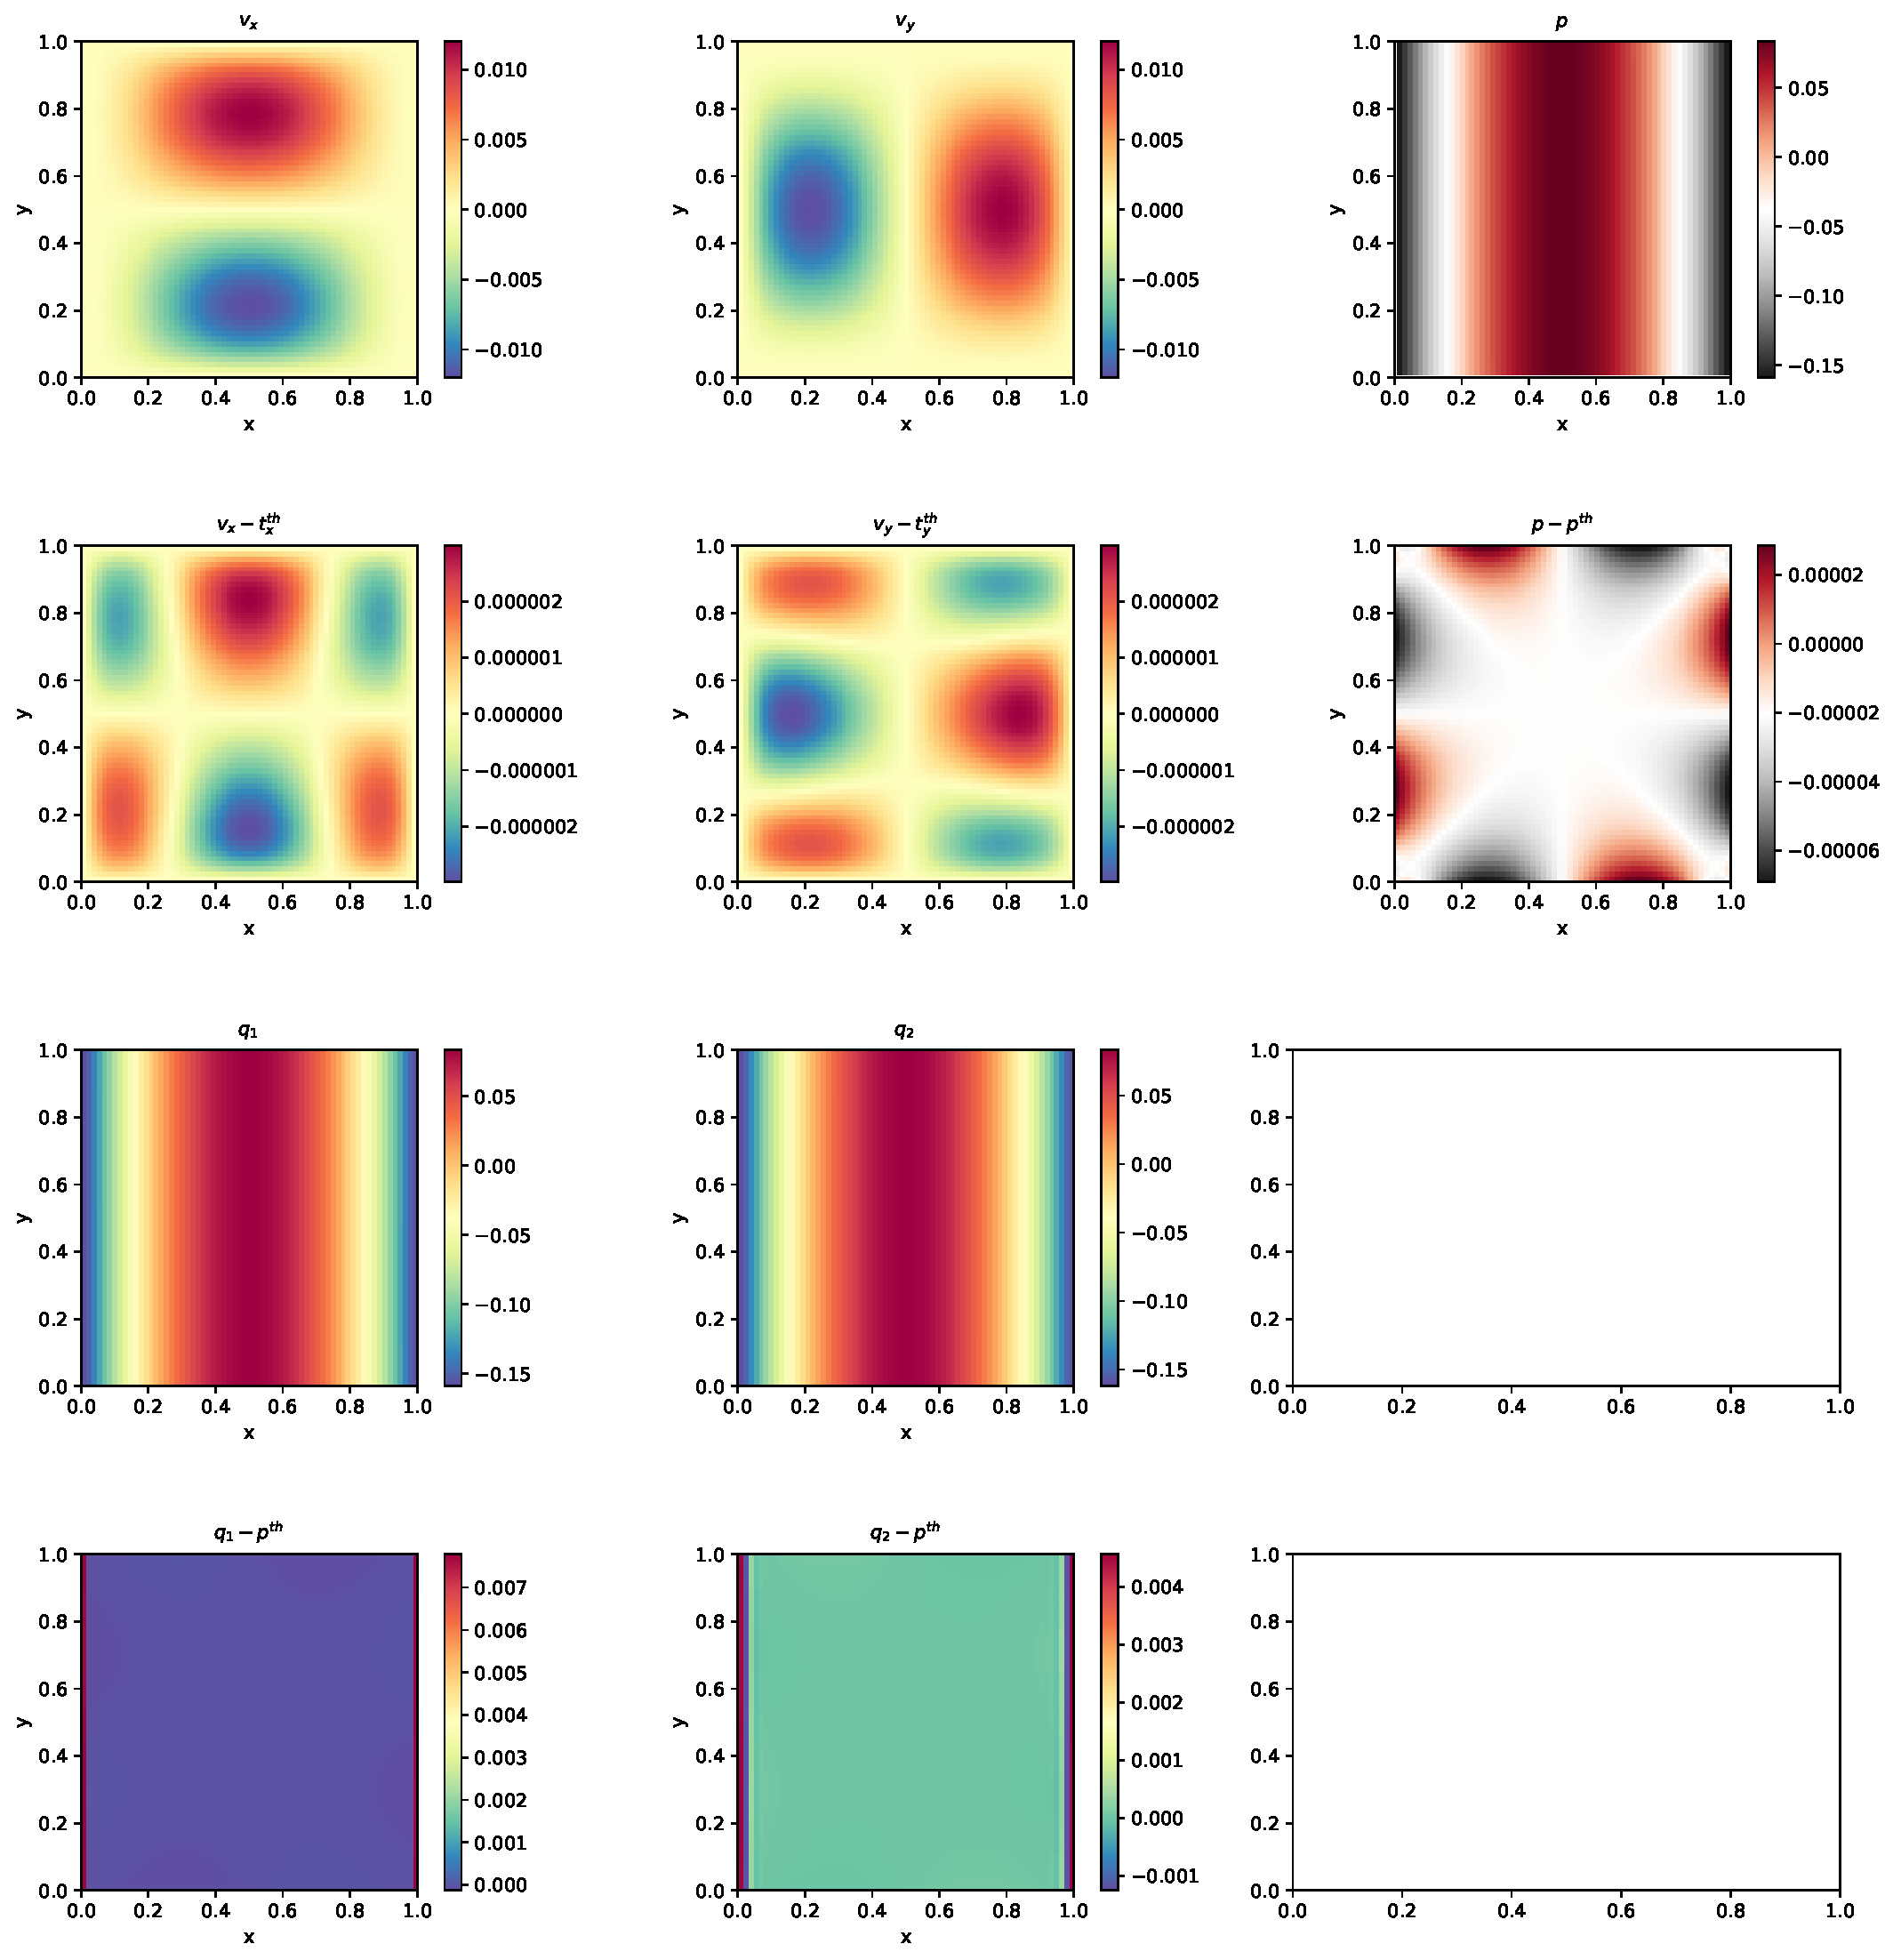
\includegraphics[width=15cm]{python_codes/fieldstone_12/solution}

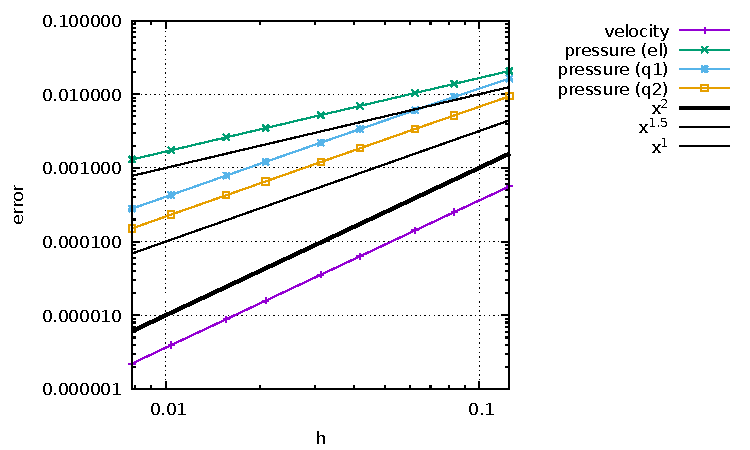
\includegraphics[width=8cm]{python_codes/fieldstone_12/errors}

In terms of pressure error, $q_2$ is better than $q_1$ which is better than elemental.

QUESTION: why are the averages exactly zero ?!

TODO: 
\begin{itemize}
\item add randomness to internal node positions.
\item look at elefant algorithms
\end{itemize}
